Two important questions can be asked about approaches like Damaris,
which propose to dedicate cores for data processing and I/O.

\begin{itemize}
\item How many dedicated cores should be used?
\item How does dedicating cores compares with dedicating nodes?
\end{itemize}

In this section we propose to answer these two questions through experiments with
the CM1 and Nek5000 simulations on Grid'5000.
We implemented in Damaris the option to use dedicated nodes instead of dedicated cores.
Some details of this implementation are given hereafter, before diving into our
experimental results.

We restrict our study to I/O. The choice of dedicating cores over dedicating nodes
for in situ visualization indeed depends on too many parameters (including the amount
of data involved, the simulation, the platform, and most importantly the visualization scenarios)
and deserves an entire study that we reserve for a future work.

\subsection{Dedicated Nodes in Damaris}

In order to compare dedicated cores with dedicated nodes, we either needed a state-of-the-art 
framework that provides dedicated nodes, such as DataSpace~\cite{dataspace}, or to 
implement dedicated nodes inside the Damaris framework. We chose the later because 
(1) our simulations are already instrumented with Damaris' API, allowing us to switch between
each approach without having to modify the simulation with another framework's API, and
(2) comparing the use of dedicated cores in Damaris with the use of dedicated nodes in
another framework would make it harder to distinguish performance benefits coming from
the approach (dedicated cores vs. dedicated nodes) from performance benefits
coming from specific optimizations of the framework itself.
This following section gives an overview of our implementation of dedicated nodes in Damaris.

\subsubsection{Implementation}

%\begin{figure*}[t]
%\centering
%	\subfigure[Writing with Dedicated Cores]{
%	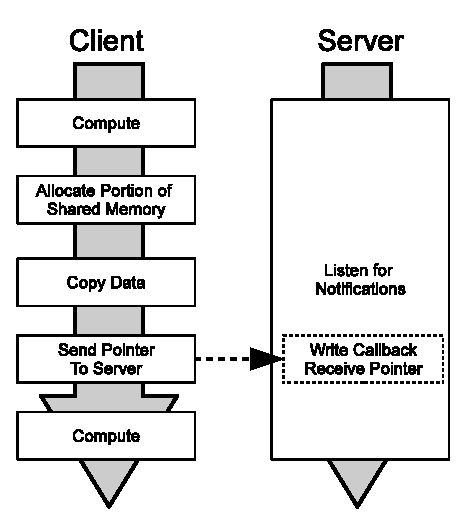
\includegraphics[width=7cm]{figures/damaris-comm-dc.eps}} 
%	\qquad
%	\subfigure[Writing with Dedicated Nodes]{
%	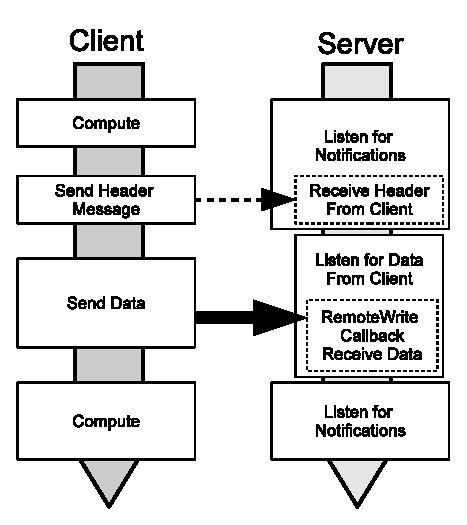
\includegraphics[width=7cm]{figures/damaris-comm-dn.eps}} 
%	%\quad
%	\subfigure[Legend]{
%	
\includegraphics[width=14cm]{figures/energy/damaris-comm-legend.eps}} 
%	\caption[Data transfer protocols using dedicated cores and dedicated nodes]{Data transfer 
%	protocols using dedicated cores and dedicated nodes.}\label{fig:io:protocols}
%\end{figure*}

The implementation of dedicated nodes in Damaris relies on asynchronous MPI communications
through Damaris' Distributed Reactor.
Each simulation core is associated with a server
running in a dedicated node. A dedicated node hosts one server on each of its cores. 
Different simulation cores may thus interact with the same dedicated node, 
but with a different core (a different server) in this node.
%The protocol used to send data from the simulation to dedicated nodes is shown in Figure~\ref{fig:io:protocol-dn}.

When a client calls \texttt{damaris\_write}, it first
sends an event to its associated server. This event triggers a \texttt{RemoteWrite} callback
in the server. When the server enters this callback, it starts a blocking \texttt{receive} to
get the data sent by the client. The client sends its data
to the server, along with metadata information such as the \emph{id} of the variable to which the data belongs.
A buffer is maintained in clients to allow these transfers to be non-blocking. When the client
needs to send data to dedicated nodes, it copies the data into this buffer and issues a non-blocking \texttt{send}
to the server using the copied data (note that this communication phase is non-blocking in clients, but blocking
on servers). The status of this operation is checked in later calls to the 
Damaris API and the buffer is freed when the transfer is completed.

Other solutions exist in the literature, for example using RDMA~\cite{docan2010enabling}
(remote direct memory access). We chose to use simple asynchronous communications for simplicity
and portability. The flexibility of our design, along with the recent addition of 
dynamic RDMA windows in the MPI~3 standard, would ease such an RDMA-based implementation 
in Damaris in a near future.

\subsubsection{``Switching Gears''}

Switching between dedicated cores and dedicated nodes, as well as changing the number of
dedicated resources, can be done through the configuration, without recompiling the
application.

\begin{itemize}
\item \verb+<dedicated cores="n" nodes="0"/>+ enables $n$ dedicated cores per node.
The number of cores per node must divide evenly into the number of dedicated cores.
\item \verb+<dedicated cores="0" nodes="n"/>+ enables $n$ dedicated nodes. 
The total number of nodes must divide evenly into the number of dedicated nodes.
\item \verb+<dedicated cores="0" nodes="0"/>+ disables dedicated cores and nodes. It triggers the time-partitioning mode.
\end{itemize}

This configuration would allow for a hybrid approach that uses
both dedicated cores and dedicated nodes. However this approach is not supported by
Damaris yet, as we haven't found any real-life scenario that would benefit from it.

The implementation of all three approaches --time partitioning, dedicated cores, dedicated nodes-- 
within the same framework allows us to evaluate their respective performance in the next sections.

%%%%%%%%%%%%%%%%%%%%%%%%%%%%%%%%%%%%%%%%%%%%%%%%%%%%%%%%%%%%%%%%%%%%%%%%%%%%%%%%
%%%%%%%%%%%%%%%%%%%%%%%%%%%%%%%%%%%%%%%%%%%%%%%%%%%%%%%%%%%%%%%%%%%%%%%%%%%%%%%%
%%%%%%%%%%%%%%%%%%%%%%%%%%%%%%%%%%%%%%%%%%%%%%%%%%%%%%%%%%%%%%%%%%%%%%%%%%%%%%%%
%%%%%%%%%%%%%%%%%%%%%%%%%%%%%%%%%%%%%%%%%%%%%%%%%%%%%%%%%%%%%%%%%%%%%%%%%%%%%%%%

\subsection{Dedicated Core(s) vs. Dedicated Nodes: an Experimental Insight}

In the following, we present the results obtained with the Nek5000 and CM1 simulations,
using the different modes in which Damaris can now operate.

\subsubsection{Results with the Nek5000 Application}

We used the MATiS configuration of Nek5000 and ran it
on 30 nodes (720 cores) of the Grid'5000's \emph{stremi} cluster. We deploy
the OrangeFS parallel file system on 4 additional nodes of this cluster.
All nodes (including the file system) communicate through a 1G Ethernet network.

Nek5000 initially writes most of its checkpoint/restart data in the form of ASCII files, 
which appeared to be highly inefficient compared to using a high-level data format such as HDF5.
We thus rewrote its I/O part as an HDF5-based plugin for Damaris, and used Damaris
in 7 configurations: without dedicated resources  (time partitioning, abbreviated TP), 
using 1, 2, or 3 dedicated cores per node (abbreviated DC(1), DC(2) and DC(3)), 
and using 2, 3 or 5 dedicated nodes (DN(14:1), DN(9:1), DN(5:1) respectively, where the notation $x:y$ represents
the ratio of computation nodes, $x$, to dedicated nodes $y$). Despite the different number of
simulation cores in each configuration, the same mesh is used as input for Nek5000 and, 
therefore, the same amount of data is produced (about 3.5~GB per iteration).
We run Nek5000 for 10 such iterations in each configuration.

\begin{figure}
	\begin{center}
	\subfigure[Average iteration time]{
		\includegraphics[width=5.5cm]{figures/damaris-nek5-runtime-tpdcdn.eps}
	}\quad
	\subfigure[Average I/O time]{
		\includegraphics[width=5.5cm]{figures/damaris-nek5-io-time-tpdcdn.eps}
	}
	\caption{Experiment with Nek5000 on 720 cores of Grid'5000 \emph{stremi} cluster. 
	Damaris is configured to use either no dedicated resources (TP), $x = $1, 2 or 3 dedicated cores (DC($x$)),
	or a ratio of $x$ computation nodes to $y$ dedicated nodes (DN($x:y$)). 
	We report (a) the average, maximum and minimum time of a single 
	iteration (computation+I/O), and (b) the average, maximum and minimum time (logarithmic scale) 
	of an I/O phase from the point of view of the simulation.}\label{fig:nek5dcdn1}
	\end{center}
\end{figure}

\paragraph{Overall run time} All configurations based on dedicated resources enable a 40\% decrease of 
overall run time compared with the time-partitioning configuration. Note that because of the inherent 
variability of the duration of the computation phases within a single iteration (represented in 
Figure~\ref{fig:nek5dcdn1} (a) by the minimum and maximum iteration times), it is not possible to tell which of 
the configuration is actually the best one.
Considering these results only, we can argue that using more dedicated cores or more dedicated nodes is 
potentially an advantageous choice (as long as the efficiency of running your simulation is not affected) 
because it offers more resources for post-processing and I/O tasks.
The choice of using dedicated cores or dedicated nodes can then be based on the characteristics of these
post-processing time (scalability, memory requirement, execution time, etc.).

\paragraph{I/O impact}
Figure~\ref{fig:nek5dcdn1} (b) shows that the duration of the I/O phase as perceived by the simulation
becomes negligible when using an approach based on dedicated resources. Dedicated cores reduce this
time down to about 0.1 seconds, while dedicated nodes reduce it to about 0.04 seconds.
This difference in communication time between dedicated cores and dedicated nodes can be easily 
explained. When using dedicated cores, the client competes with other clients for the access to a 
mutex-protected segment of shared memory. When using dedicated
nodes on the other hand, this contention does not occur, as each client simply makes a local copy 
of its data and issues a non-blocking send that proceeds in parallel with the simulation. 
Therefore, while the I/O phase appears faster with dedicated nodes, our results do not show the potential
impact that background communications with dedicated nodes may have on the performance of the simulation.

\begin{figure}
	\begin{center}
	\subfigure[Average aggregate throughput]{
		\includegraphics[width=5.5cm]{figures/damaris-nek5-throughput-tpdcdn.eps}
	}\quad
	\subfigure[Spare time in dedicated resources]{
		\includegraphics[width=5.5cm]{figures/damaris-nek5-spare-tpdcdn.eps}
	}
	\caption{Experiment with Nek5000 on 720 cores of Grid'5000 \emph{stremi} cluster. 
	Damaris is configured to use either no dedicated resources (TP), $x = $1, 2 or 3 dedicated cores (DC($x$)),
	or a ratio of $x$ computation nodes to $y$ dedicated nodes (DN($x:y$)). 
	We report (a) the average, maximum and minimum aggregate throughput
	from writer processes, and (b) the spare time in dedicated processes for the approaches that leverage them.}\label{fig:nek5dcdn2}
	\end{center}
\end{figure}

\paragraph{Aggregate throughput}
From the point of view of writer processes (or from the point of view of the file system),
the different configurations lead to different aggregate throughput. Figure~\ref{fig:nek5dcdn2} (a) shows that
dedicated cores achieve the highest throughput. This throughput is slightly degraded as the number of
dedicated cores per node increases, due to contention between dedicated cores on the same node.
Dedicated nodes also increase the aggregate throughput compared with time partitioning, but do not achieve
the throughput of dedicated cores. This is due to the fact that all cores in dedicated nodes are writing,
and thus compete for the network access at the level of each single dedicated nodes.
Additionally, the lower throughput observed when using only two dedicated nodes can be explained
by the fact that the file system features four data servers. Therefore, dedicating only two nodes does not
fully take advantage of parallelism across writers.

\paragraph{Spare time}
Finally, Figure~\ref{fig:nek5dcdn2} (b) shows the spare time in dedicated resources. In all configurations
based on dedicated cores, the dedicated cores spend 10\% of their time writing, and remain idle 90\% of the time.
Dedicated nodes spend slightly more time writing (from 13 to 20\% of their time). This is a direct consequence
of the difference in aggregate throughput.

\paragraph{Conclusion}
Overall, all the configurations based on dedicated resources improve the simulation run time in a similar way.
These configurations however differ in other aspects. By avoiding contention at the level of a node, 
dedicated cores achieve a higher throughput and
therefore spare more time that can be used for data processing. Yet, if we weight this spare time
by the number of cores that can be used to leverage it (90 when dedicating 3 cores per node, 120 when
dedicating 5 nodes), the configuration based on 5 dedicated nodes appears to spare more resources (core-seconds)
in spite of sparing less time per core.

The choice of whether one should use an approach based on dedicated cores or dedicated nodes is of
course not restricted to these considerations. Some memory-bound simulations may not be able to afford 
allocating shared memory to dedicated cores, and would rather benefit from dedicated nodes. 
Some I/O intensive simulations on the other hand may not be able to transfer large amounts of data 
to a reduced number of dedicated nodes and will prefer dedicated cores.

\subsubsection{Results with the CM1 application}

In this section, we leverage experiments with the CM1 simulation to show that the choice of one 
approach over another also depends on the platform considered.

We used CM1 on Grid'5000's Nancy and Rennes sites.
On the Nancy site we use the \emph{graphene} cluster. Each node of this cluster consists of a 4-core
Intel Xeon 2.53~GHz CPU with 16~GB of RAM. Intra-cluster communication is done through a 1G Ethernet network.
A 20G InfiniBand network is used between these nodes and the OrangeFS file system deployed on 6 I/O servers.

On the Rennes site we use the \emph{parapluie} cluster, already presented in Section~\ref{sec:expIO}. 
The nodes communicate with one another through a 1G Ethernet network and with an OrangeFS file system
deployed on 3 servers across a 20G InfiniBand network.

We deploy CM1 on 32 nodes (128 cores) on the Nancy site. On the Rennes site, we deploy it on 16 nodes (384 cores).
In both cases, we configure CM1 to complete 2520 time steps. We vary its output frequency, using 10, 20 or 30 time steps
between each output. Damaris is configured to run with CM1 in five different scenarios that cover the three I/O approaches
considered: time partitioning, dedicated cores (one or two -- DC(1) and DC(2)), and dedicated
nodes using a ratio of 7:1 (DN(7:1), 7 compute nodes for one dedicated node) or 15:1 (DN(15:1), 15 compute nodes for one dedicated
node). DN(7:1) thus uses four dedicated nodes on the Nancy site, two on the Rennes site. DN(15:1) dedicates two nodes
on the Nancy site, one on the Rennes site.

\begin{figure}
	\begin{center}
	\subfigure[Run time of CM1 on Nancy cluster]{
		\includegraphics[width=5.5cm]{figures/nancy-cm1-runtime.eps}
	}\quad
	\subfigure[Run time of CM1 on Rennes cluster]{
		\includegraphics[width=5.5cm]{figures/rennes-cm1-runtime.eps}
	}
	\caption{Experiment with CM1 on Grid'5000 Rennes (24 cores per node) and Nancy (4 cores per node) sites. 
	Damaris is configured to use either no dedicated resources (TP), $x = $1 or 2 dedicated cores (DC($x$)),
	or a ratio of 7:1 or 15:1 dedicated nodes (DN(7:1) and DN(15:1)). We report total run time for 2520 time steps.}\label{fig:cm1dcdn}
	\end{center}
\end{figure}

\paragraph{Impact of the platform} Figure~\ref{fig:cm1dcdn} shows that in both clusters, dedicating resources drastically 
improve the performance of CM1 compared with a time-partitioning approach. 
Dedicating four nodes on Nancy enables an almost $3\times$ overall speedup, while
dedicating one core in each node on the Rennes cluster leads to more than $5\times$ speedup.
Our results also show that the best approach in terms of overall run time depends on the platform. It consists of 
using dedicated nodes with a 7:1 ratio on the Nancy cluster, and using one dedicated core per node on the Rennes cluster. 
This conclusion is not surprising, since the Nancy cluster only provides 4 cores per node. Dedicating some of these
cores thus has a large impact on the simulation. On the Rennes cluster, which provides 24 cores per node, dedicating
some of these cores does not remove such an important fraction of computational power from the simulation and is
thus more efficient than dedicating nodes.

\subsection{Conclusion}

Over the years, several research groups have proposed new approaches to I/O and data processing
based on dedicated resources. These approaches can be divided into a group of approaches based on dedicated
cores, and a group of approaches based on dedicated nodes. While Damaris was initially part of the first one,
we extended it to support a wider range of configurations. It now offers to dedicate either a subset of cores
in each multicore node, or entire nodes. Additionally, it also offers to not dedicate any resource at all,
performing all data processing and movement synchronously. This flexibility, made possible in particular
through a configuration file that allows us to switch between modes very easily, let us to compare these
approaches.

Our results show that dedicating resources for I/O is a highly efficient method to improve the I/O performance
of a simulation, both in terms of overall run time, aggregate throughput and performance variability. 
They also highlighted the fact that there is no clear advantage of one approach over the other: 
dedicating cores appears more efficient than dedicated nodes under certain conditions, and the opposite holds 
under different conditions. The choice
of one approach over the other may also depend on criteria other than the overall run time. Our experiments
with Nek5000 showed that while this run time is very similar under the different approaches, the resulting
aggregate throughput favors dedicating cores, while the resulting spared resources (spare time $\times$ number 
of cores in dedicated resources) advocates for using dedicated nodes. Our experiments with CM1 showed that
the choice of one approach over the other also depends on the platform. While an approach based on dedicated cores is
more suitable on a platform featuring a large number of cores per node, it may be more efficient to use dedicated nodes
on a platform with a reduced number of cores per node.
